\documentclass[]{article}
\usepackage{lmodern}
\usepackage{amssymb,amsmath}
\usepackage{ifxetex,ifluatex}
\usepackage{fixltx2e} % provides \textsubscript
\ifnum 0\ifxetex 1\fi\ifluatex 1\fi=0 % if pdftex
  \usepackage[T1]{fontenc}
  \usepackage[utf8]{inputenc}
\else % if luatex or xelatex
  \ifxetex
    \usepackage{mathspec}
  \else
    \usepackage{fontspec}
  \fi
  \defaultfontfeatures{Ligatures=TeX,Scale=MatchLowercase}
\fi
% use upquote if available, for straight quotes in verbatim environments
\IfFileExists{upquote.sty}{\usepackage{upquote}}{}
% use microtype if available
\IfFileExists{microtype.sty}{%
\usepackage{microtype}
\UseMicrotypeSet[protrusion]{basicmath} % disable protrusion for tt fonts
}{}
\usepackage[unicode=true]{hyperref}
\hypersetup{
            pdftitle={Linked Data Notifications: a resource-centric communication protocol},
            pdfborder={0 0 0},
            breaklinks=true}
\urlstyle{same}  % don't use monospace font for urls
\usepackage{graphicx,grffile}
\makeatletter
\def\maxwidth{\ifdim\Gin@nat@width>\linewidth\linewidth\else\Gin@nat@width\fi}
\def\maxheight{\ifdim\Gin@nat@height>\textheight\textheight\else\Gin@nat@height\fi}
\makeatother
% Scale images if necessary, so that they will not overflow the page
% margins by default, and it is still possible to overwrite the defaults
% using explicit options in \includegraphics[width, height, ...]{}
\setkeys{Gin}{width=\maxwidth,height=\maxheight,keepaspectratio}
\IfFileExists{parskip.sty}{%
\usepackage{parskip}
}{% else
\setlength{\parindent}{0pt}
\setlength{\parskip}{6pt plus 2pt minus 1pt}
}
\setlength{\emergencystretch}{3em}  % prevent overfull lines
\providecommand{\tightlist}{%
  \setlength{\itemsep}{0pt}\setlength{\parskip}{0pt}}
\setcounter{secnumdepth}{0}
% Redefines (sub)paragraphs to behave more like sections
\ifx\paragraph\undefined\else
\let\oldparagraph\paragraph
\renewcommand{\paragraph}[1]{\oldparagraph{#1}\mbox{}}
\fi
\ifx\subparagraph\undefined\else
\let\oldsubparagraph\subparagraph
\renewcommand{\subparagraph}[1]{\oldsubparagraph{#1}\mbox{}}
\fi

\title{Linked Data Notifications: a resource-centric communication protocol}
\date{}

\begin{document}
\maketitle

\section{Linked Data Notifications: a resource-centric communication
protocol}\label{linked-data-notifications-a-resource-centric-communication-protocol}

\hypertarget{authors}{}
\begin{description}
\tightlist
\item[Authors]
{{\href{http://csarven.ca/}{{{Sarven}
{Capadisli}}}}}\textsuperscript{\protect\hyperlink{author-org-1}{1}\protect\hyperlink{author-email-1}{✊}}

{{\href{https://rhiaro.co.uk/}{{{Amy}
{Guy}}}}}\textsuperscript{\protect\hyperlink{author-org-2}{2}\protect\hyperlink{author-email-2}{🐦}}

{\href{https://langec.wordpress.com/about/}{Christoph
Lange}}\textsuperscript{\protect\hyperlink{author-org-1}{1}\protect\hyperlink{author-email-3}{∫}}

{\href{http://eis.iai.uni-bonn.de/SoerenAuer.html}{Sören
Auer}}\textsuperscript{\protect\hyperlink{author-org-1}{1}\protect\hyperlink{author-email-4}{⚛}}

{\href{https://www.w3.org/People/Berners-Lee/}{Tim
Berners-Lee}}\textsuperscript{\protect\hyperlink{author-org-4}{3}\protect\hyperlink{author-email-5}{🕸}}
\end{description}

\begin{itemize}
\item
  \hypertarget{author-org-1}{}

  \textsuperscript{1}Enterprise Information Systems Department,
  \href{http://uni-bonn.de/}{University of Bonn}, Bonn, DE
\item
  \hypertarget{author-org-2}{}

  \textsuperscript{2}School of Informatics,
  \href{http://inf.ed.ac.uk/}{University of Edinburgh}, Edinburgh, UK
\item
  \hypertarget{author-org-3}{}

  \textsuperscript{3}Decentralized Information Group, CSAIL,
  \href{https://mit.edu/}{MIT}, Cambridge, US
\end{itemize}

\begin{itemize}
\item
  \hypertarget{author-email-1}{}

  \textsuperscript{✊}\href{mailto:info@csarven.ca}{\nolinkurl{info@csarven.ca}}
\item
  \hypertarget{author-email-2}{}

  \textsuperscript{🐦}\href{mailto:amy@rhiaro.co.uk}{\nolinkurl{amy@rhiaro.co.uk}}
\item
  \hypertarget{author-email-3}{}

  \textsuperscript{∫}\href{mailto:langec@cs.uni-bonn.de}{\nolinkurl{langec@cs.uni-bonn.de}}
\item
  \hypertarget{author-email-4}{}

  \textsuperscript{⚛}\href{mailto:auer@cs.uni-bonn.de}{\nolinkurl{auer@cs.uni-bonn.de}}
\item
  \hypertarget{author-email-5}{}

  \textsuperscript{🕸}\href{mailto:timbl@w3.org}{\nolinkurl{timbl@w3.org}}
\end{itemize}

\hypertarget{content}{}
\hypertarget{abstract}{}
\subsection{Abstract}\label{abstract}

In this article we describe the Linked Data Notifications (LDN)
protocol, which is a \href{https://www.w3.org/TR/ldn/}{W3C Candidate
Recommendation}. Notifications are sent over the Web for a variety of
purposes, for example, by social applications. The information contained
within a notification is structured arbitrarily, and typically only
usable by the application which generated it in the first place. In the
spirit of Linked Data, we propose that notifications should be reusable
by multiple authorised applications. Through separating the concepts of
\emph{senders}, \emph{receivers} and \emph{consumers} of notifications,
and leveraging Linked Data principles of shared vocabularies and URIs,
LDN provides a building block for decentralised Web applications. This
permits end users more freedom to switch between the online tools they
use, as well as generating greater value when notifications from
different sources can be used in combination. We situate LDN alongside
related initiatives, and discuss additional considerations such as
security and abuse prevention measures. We evaluate the protocol's
effectiveness by analysing multiple, independent implementations, which
pass a suite of formal tests and can be demonstrated interoperating with
each other. To experience the described features please open this
document in your Web browser under its canonical URI:
http://csarven.ca/linked-data-notifications

\hypertarget{keywords}{}
\subsection{Keywords}\label{keywords}

\begin{itemize}
\tightlist
\item
  \href{https://en.wikipedia.org/wiki/Communications_protocol}{Communications
  protocol}
\item
  \href{https://en.wikipedia.org/wiki/Decentralization}{Decentralisation}
\item
  \href{https://en.wikipedia.org/wiki/Linked_data}{Linked Data}
\item
  \href{https://en.wikipedia.org/wiki/Social_web}{Social web}
\end{itemize}

\hypertarget{introduction}{}
\subsection{Introduction}\label{introduction}

Notifications are sent over the Web for a variety of purposes, including
social applications: ``You have been invited to a graduation party!'',
``Tim commented on your blog post!'', ``Liz tagged you in a photo''. The
notification data may be displayed to a human to acknowledge, or used to
trigger some other application-specific process (or both).
\protect\hypertarget{issue}{}{In a decentralised architecture,
notifications can be a key element for federation of information, and
application integration. However in {centralised systems which prevail
today}, this data is structured arbitrarily and typically only usable by
the application that generated it in the first place. Current efforts
towards \emph{re-decentralising} the Web
{[}\protect\hyperlink{ref-1}{1}, \protect\hyperlink{ref-2}{2},
\protect\hyperlink{ref-3}{3}{]} are moving towards architectures in
which data storage is decoupled from application logic, freeing end
users to switch between applications, or to let multiple applications
operate over the same data. So far, notifications are considered to be
\emph{ephemeral} resources which may disappear after transport, and thus
are excluded from being designed for reuse.}

We argue that notification data should not be locked into particular
systems. We designed the \emph{Linked Data Notifications (LDN)} protocol
to support sharing and reuse of notifications \emph{across}
applications, regardless of how they were generated or what their
contents are. We describe how the principles of identification,
addressability and semantic representation can be applied to
notifications on the Web. Specifying LDN as a formal protocol allows
independently implemented, heterogeneous applications which generate and
use notifications, to seamlessly work together. Thus, LDN supports the
decentralisation of the Web as well as encourages the generation and
consumption of Linked Data.

We build on existing W3C standards and Linked Data principles. In
particular, the storage of notifications is compatible with the Linked
Data Platform standard; notifications are identified by HTTP URIs; and
notification contents are available as JSON-LD. A key architectural
decision is the separation of concerns between \emph{senders},
\emph{receivers}, and \emph{consumers} of notifications. Implementations
of the protocol can play one or more of these roles, and interoperate
successfully with implementations playing the complementary roles. This
means that notifications generated by one application can be reused by a
completely different application, accessed via the store where the
notification data resides, through shared Linked Data vocabularies. LDN
also pushes the decentralised approach further by allowing any
\emph{target} resource to advertise its Inbox anywhere on the Web; that
is, targets do not need to be coupled to or controlled by a receiver,
and can make use of a third-party \emph{Inbox as a service}.{}

LDN is a W3C \href{https://www.w3.org/TR/ldn/}{Candidate Recommendation}
via the \href{https://www.w3.org/wiki/Socialwg}{Social Web Working
Group} {[}\protect\hyperlink{ref-4}{4}{]}. The first two authors of this
article are the co-editors of the specification.

Use cases for decentralised notifications are particularly evident in
social networking (status updates, interactions, games); scholarly
communication (reviews, citations); and changes of state of resources
(datasets, versioning, sensor readings, experimental observations). We
describe the requirements which guided the development of the protocol
and discuss related work, including current alternative approaches and
complementary protocols which can work alongside LDN. We summarise the
protocol itself, and specific architectural considerations that were
made. We built a test suite which can be used to confirm that
implementations conform with the specification, and we describe 17
implementations which interoperate with each other.

\hypertarget{concept-scheme}{}
{As the following terms used throughout this article may be subject to
different interpretations by different communities, we provide some
definitions here.}

By \textbf{decentralisation}, we mean {data and applications are loosely
coupled, and users are empowered to choose where their data is stored or
held. We focus on Web-based decentralisation, where content is
transported over HTTP, and resources are identified with URIs.} An
\textbf{Inbox} is {a container or directory (attached to a Web resource)
which is used to store and serve a collection of notifications.} A
\textbf{notification} is {a retrievable resource which returns RDF. The
contents of notifications are intended to describe a change in state of
some other resource, or contain new information for the attention of a
user or process, and may be subject to constraints of the Inbox it is
contained in.}

\hypertarget{related-work}{}
\subsection{Related Work}\label{related-work}

Here we review previous and ongoing efforts towards delivering
notifications in a decentralised manner. Many systems which make use of
notifications operate either in a completely centralised way, or are
decentralised only in the sense that different instances of the
\emph{same} codebase need to interoperate; we restrict our review to
mechanisms which do not expect the notification to be received or used
only by the same software or platform which sent it.

The contents of a notification is either: 1) URLs, indicating relations
between Web resources, or 2) a `fat ping' containing a blob of
information. Semantic Pingback, Webmention, and Provenance Pingback
follow the first form, and are also known as linkbacks, the suite of
protocols that essentially allows Web documents to automatically
reciprocate hyperlinks. This has the advantage that a verification
mechanism can be tightly specified (the URL of the target must appear in
the content of the source), but the disadvantage that notifications are
only available for use cases involving Web publishing.

\href{https://aksw.github.io/SemanticPingback/}{Semantic Pingback}
{[}\protect\hyperlink{ref-2}{2}{]} and
\href{https://www.w3.org/TR/webmention}{Webmention}
{[}\protect\hyperlink{ref-5}{5}{]} both update the original
\href{http://www.hixie.ch/specs/pingback/pingback}{Pingback}
{[}\protect\hyperlink{ref-6}{6}{]} mechanism by replacing the XML-RPC
transport mechanism by a \texttt{x-www-form-urlencoded} request with two
parameters (\texttt{source} and \texttt{target}). Resources which are
the target for a notification advertise the respective receiving service
or endpoint via a \texttt{Link} relation, either in HTTP headers or
HTML. Semantic Pingback additionally enables discovery of the Pingback
service where target is available as RDF. While the content at source
may indicate (in any convention or serialisation format) the type of
relation between the source and target URLs, this information about the
relation is not transmitted to the receiver's endpoint; only the source
and target URLs are sent. As such, there is also no way to distinguish
between multiple potential mentions of the target at the source; this is
left up to the receiver to interpret. Semantic Pingback does encourage
generation of additional semantics about the relation(s) between the
source and the target by processing the source as RDF if possible, and
also defines specific ways for a receiving server to handle incoming
pingback data in order to add the source data to an RDF knowledge base
{[}\protect\hyperlink{ref-2}{2}{]}. Beyond verifying that the source
contains the URL of the target, Webmention does not specify any further
requirements of the receiving server; nor is it expected that
``mentions'' are retrievable once they have been sent.

A \href{http://www.w3.org/TR/prov-aq/\#provenance-pingback}{Provenance
Pingback} endpoint is also advertised via the HTTP \texttt{Link} header;
it accepts a list of URIs for provenance records describing uses of the
resource {[}\protect\hyperlink{ref-7}{7}{]}. Provenance Pingback does
not specify any further behaviour by the receiving server, but the
contents at the URIs listed in the notification body must be semantic
data.

Other notification mechanisms send more information than just URLs in
the notification body; due to each mechanism's focused use case, the
payload is restricted to a particular vocabulary.

\href{http://www.cibiv.at/~niko/dsnotify/}{DSNotify} is a centralised
service which crawls datasets and observes changes to links with the
specific use case of preserving link integrity between Linked Open Data
resources. Third-party applications can register with the sending
service to receive notifications of changes in the form of a specific
XML payload {[}\protect\hyperlink{ref-8}{8}{]}. With the
\href{https://www.w3.org/2001/sw/wiki/SparqlPuSH}{sparqlPuSH} service,
users may input a SPARQL query, the results of which are the specific
updates they are interested in. The query is run periodically by the
service, and the results are converted to RSS and Atom feeds, which is
sent to a
\href{http://pubsubhubbub.github.io/PubSubHubbub/pubsubhubbub-core-0.4.html}{PubSubHubbub}
hub to which the user can subscribe {[}\protect\hyperlink{ref-9}{9}{]}.
The
\href{http://www.openarchives.org/rs/notification/1.0/notification}{ResourceSync
Change Notification} specification also sends update notifications via a
PuSH hub, this time with an XML payload based on the Sitemap format
{[}\protect\hyperlink{ref-10}{10}{]}. Each of these mechanisms is
triggered by subscription requests. That is, a user must actively
solicit messages from a particular service, rather than having a way for
a service to select a notification target and autonomously discover
where to send notifications to.

\hypertarget{requirements-and-design-considerations}{}
\hypertarget{requirements-and-design-considerations}{\subsection{Requirements
and Design
Considerations}\label{requirements-and-design-considerations}}

In this section we discuss our considerations for a {Web notification
protocol that conforms to the Linked Data design principles}, as well as
{best practices for applications}. We use these considerations to
establish both concrete requirements and points of
implementation-specific flexibility for the protocol.

\hypertarget{modularity}{}
\subsubsection{R1 Modularity}\label{r1-modularity}

To encourage modularity of applications, one should differentiate
between different classes of implementation of the protocol. Two parties
are involved in the creation of a notification: a \emph{sender},
generating the notification data, and a \emph{receiver}, storing the
created resource. We also have the role of a \emph{consumer}, which
reads the notification data and repurposes it in some way. A software
implementation can of course play two or all three of these roles; the
important part is that it need not. A consuming application can read and
use notification data without being concerned about ever sending or
storing notifications.

\hypertarget{reusable-notifications}{}
\subsubsection{R2 Reusable
notifications}\label{r2-reusable-notifications}

The relationship between the \emph{consumer} and \emph{receiver} roles
is key to notifications being reusable. A consumer must be able to
autonomously find the location of notifications for or about the
particular resource it is interested in. To achieve this we place a
requirement on the receiver to expose notifications it has been sent in
such away to permit other applications to access them; and specify how
any resource can advertise its receiving endpoint for consumers to
discover. To promote fair use or remixing of notification contents,
applications can incorporate rights and licensing information into the
data. Similarly, applications may include additional information on
licensing resources that the notification refers to. The presence of
this type of information is important for consumers to assess the
(re)usability of data.

\hypertarget{persistence-and-retrievability}{}
\subsubsection{R3 Persistence and
Retrievability}\label{r3-persistence-and-retrievability}

There is a social expectation and technical arguments for ensuring the
persistence of identifiers of Web resources
{[}\protect\hyperlink{ref-11}{11}{]}. This is inconsistent with the
traditionally ephemeral nature of notifications. Applications may
benefit from referring to or reusing notifications if the notifications
are known to be available in the long term, or indicate their expected
lifespan {[}\protect\hyperlink{ref-12}{12}{]}.

A \emph{RESTful architecture} {[}\protect\hyperlink{ref-13}{13}{]} is
well suited for persistent notifications, as it involves organisation of
atomic resources, their discovery and description, and a lightweight API
for the CRUD (create, read, update, and delete) operations
{[}\protect\hyperlink{ref-14}{14}{]}. This enforces the notion that
notifications are considered resources in their own right, with their
own dereferencable URIs.

We need to consider both the needs of software systems and humans when
large amounts of notification data are being generated and shared
between diverse applications which may be operating without knowledge of
each other. To organise and manage large amount of notifications over
time, mechanisms should be in place to break representations of
collections of notifications into multiple paged responses that may be
easier to consume by applications.

Relatedly, receivers may carry out resource management or garbage
collection, or permit consumers or other applications to do so. For
example, an application to consume messages might let an authenticated
and authorised user `mark as read' by adding a triple to the
notification contents.

\hypertarget{adaptability}{}
\subsubsection{R4 Adaptability}\label{r4-adaptability}

Linked Data applications benefit from domain-driven designs; that is,
functionality being small and focussed on a particular purpose, rather
than generic. We believe a notification protocol should be adaptable for
different domains, but that there is no need to create multiple
domain-specific notification protocols; the fundamental mechanics are
the same.

\textbf{R4-A}: Any resource may be the \emph{target} of a notification.
By target, we mean a notification may be addressed \emph{to} the
resource, be \emph{about} the resource, or for a sender to otherwise
decide that it is appropriate to draw the attention of the resource (or
resource owner) to the information in the notification body. As such,
any Web resource must be able to advertise an endpoint to which it can
receive notifications. Resources can be RDF or non-RDF (such as an
image, or CSV dataset), and may be informational (a blog post, a user
profile) or non-informational (a person).

\textbf{R4-B}: We do not purport to be able to design a notifications
ontology which is appropriate for every domain. Thus we consider the
\emph{contents} of a notification to be application specific. From a
sender's perspective, we derive two core principles: a notification can
contain \emph{any data}; a notification can use \emph{any vocabulary}.
From a consumer's perspective, interoperability between different
applications occurs through vocabulary reuse, and shared understanding
of terms. This is in accordance with Linked Data principles in general.
The practical upshot of this is that a calendar application which
consumes event invitations using the
\href{https://www.w3.org/TR/rdfcal/}{RDF Calendar} vocabulary is likely
to completely ignore notifications containing the
\href{www.w3.org/TR/prov-o/}{PROV Ontology}, even if it finds them all
stored in the same place. For two independent applications operating in
the \emph{same} domain, a shared understanding of appropriate vocabulary
terms is assumed.

\hypertarget{notification-verification}{}
However from a receiver's perspective, exposing itself to receive any
blobs of RDF data from unknown senders may be problematic. Thus,
\textbf{R4-C}: it should be possible for the receiver to enforce
restrictions and accept only notifications that are acceptable according
to its own criteria (deemed by e.g., user configuration; domain-specific
receivers). This can be used as an anti-spam measure, a security
protection, or for attaining application and data integrity.

Rejecting notifications which do not match a specific pattern in their
contents, or the \emph{shape} of the data, is one way to filter. For
example, if the Inbox owner knows that they will only ever use a
consuming application which processes friend requests, they can
configure their receiver to filter out anything that does not match the
pattern for a friend request, helping their consumer to be more
efficient. If the notification constraints are also advertised by the
receiving service as structured descriptions, generation and consumption
of the notifications can be further automated. Possible specifications
for doing so are W3C \href{https://www.w3.org/TR/shacl/}{Shapes
Constraint Language (SHACL)} {[}\protect\hyperlink{ref-15}{15}{]} or
\href{https://shexspec.github.io/spec/}{ShEx}.

Receivers may wish to filter notifications by verifying the sender,
through for example a whitelist or a Web of trust. This requires an
authentication mechanism and since different authentication mechanisms
are appropriate for different applications, the notification protocol
should ideally be usable alongside various methods such as clientside
certificates, e.g., WebID+TLS, token-based, e.g., OAuth 2.0, or digital
signatures.

As ``anyone can say anything about anything'' a receiver may choose to
resolve any external resources referred to by the notification, and
cross-check the notification contents against authoritative sources.
This is similar to how Semantic Pingback and Webmention require fetching
and parsing of the source URL to verify existence of the target link.

\hypertarget{subscribing}{}
\subsubsection{R5 Subscribing}\label{r5-subscribing}

In general, applications may require that new notifications are pushed
to them in real-time, or to request them at appropriate intervals. To
take this into account, we expand our definition of senders, receivers
and consumers with the following interaction expectations: notifications
are \emph{pushed} from senders to receivers; and \emph{pulled} from
receivers by consumers.

Thus, an application which offers an endpoint or callback URL to which
notifications should be sent directly is a receiver, and an application
which fetches notifications from an endpoint on its own schedule is a
consumer. Much of the related work \emph{requires} notifications to be
explicitly solicited to trigger sending. Since in a decentralised model,
receivers may not be aware of possible sources for notifications, our
sender-receiver relationship depends on the sender's autonomy to make
such decisions by itself. This does not preclude the scenario in which a
receiver may wish to solicit notifications from a particular sender, but
as there are already subscription mechanisms in wide use on the Web, we
do not need to specify it as part of LDN. For example,
\href{https://www.w3.org/TR/websub/}{WebSub} (recent W3C evolution of
PubSubHubbub), the WebSocket Protocol, or HTTP Web Push.

Given our adoption of Linked Data principles and a RESTful architecture,
a further design decision was to ensure minimal compatibility with the
\href{https://www.w3.org/TR/ldp/}{Linked Data Platform} (LDP)
specification {[}\protect\hyperlink{ref-16}{16}{]}. LDP is a RESTful
read-write API for RDF resources, which groups related resources
together into constructs known as ``Containers''. Thus, existing LDP
servers can be used to store notifications, as new notifications can be
created by \texttt{POST}ing RDF to a container.

\hypertarget{protocol}{}
\subsection{The LDN Protocol}\label{the-ldn-protocol}

The Linked Data Notifications (LDN) protocol describes how servers
(receivers) can receive messages pushed to them by applications
(senders), as well as how other applications (consumers) may retrieve
those messages. Any resource can advertise a receiving endpoint (Inbox)
for notification messages. Messages are expressed in RDF, and can
contain arbitrary data. It is not dependent on a complete implementation
of LDP, but comprises an easy-to-implement subset. LDN is a
\href{https://www.w3.org/TR/ldn}{W3C Candidate Recommendation}
{[}\protect\hyperlink{ref-4}{4}{]}.

Overview of Linked Data Notifications

\hypertarget{sender-to-receiver}{}
\subsubsection{Sender to receiver
interactions}\label{sender-to-receiver-interactions}

The following steps (in order without skipping) describe the interaction
between sender and receiver:

(1) A sender is triggered, either by a human or an automatic process, to
deliver a notification; (2) The sender chooses a target resource to send
notifications to; (3) The sender discovers the location of the target's
\emph{Inbox} through the \texttt{ldp:inbox} relation in the HTTP
\texttt{Link} header or RDF body of the target resource; (4) The sender
creates the body of the notification according to the needs of
application; (5) The sender makes a \texttt{POST} to the Inbox URL,
containing the body in JSON-LD or in another serialisation acceptable by
the server; (6) The receiver optionally applies filtering rules, and
sends the appropriate HTTP response code to accept or reject the
notification; (7) The receiver exposes the notification data (according
to appropriate access control) for use by consumers.

\hypertarget{consumer-to-receiver}{}
\subsubsection{Consumer to receiver
interactions}\label{consumer-to-receiver-interactions}

The following steps (in order without skipping) describe the interaction
between consumer and receiver:

(1) A consumer selects a target and discovers the location of its Inbox
in the same way as the sender; (2) A receiver responds to \texttt{GET}
requests made to the Inbox URL with a listing of the URLs of
notifications that have previously been accepted, linked to the Inbox
with the \texttt{ldp:contains} predicate; {(3) The receiver responds to
\texttt{GET} requests made to the individual notification URLs with
JSON-LD (or optionally other serialisations);} {(4) Following the
retrieval of notification listings or individual notifications, the
consumer may perform further processing, combine with some other data,
or simply present the results in a suitable human-readable way.}

\hypertarget{example-notifications}{}
\subsubsection{Example Notifications}\label{example-notifications}

For more example notification payloads, see the
\href{https://www.w3.org/TR/ldn/}{LDN specification}.

\begin{verbatim}
{
  "@context": { "sioc": "http://rdfs.org/sioc/ns#" }
  "@id": "",
  "@type": "sioc:Comment",
  "sioc:content": "This is a great article!",
  "sioc:reply_of": { "@id": "http://example.org/article" },
  "sioc:created_at": { "@value": "2015-12-23T16:44:21Z" }
}
\end{verbatim}

A notification about a comment created by a user (JSON-LD).

\begin{verbatim}
@prefix as: <https://www.w3.org/ns/activitystreams#> .
@prefix cito: <http://purl.org/spar/cito/> .
<> a as:Announce
  as:object <https://linkedresearch.org/resources#r-903b83> ;
  as:target <http://csarven.ca/dokieli#architecture> .
<https://linkedresearch.org/resources#r-903b83>
  cito:citesAsPotentialReading
    <http://csarven.ca/linked-data-notifications#protocol> .
\end{verbatim}

An announcement of a specific citation relation between two entities
(Turtle).

\hypertarget{implementations}{}
\hypertarget{implementations}{\subsection{Implementations}\label{implementations}}

Here we summarise the 17 LDN implementations we are aware of to date.
They are built by 10 different teams or individuals using different tool
stacks (5 clientside JavaScript, 3 PHP, 3 NodeJS, 3 Python, 1 Perl, 1
Virtuoso Server Pages, 1 Java) and have submitted
\href{https://github.com/w3c/ldn/tree/master/implementations}{implementation
reports} as part of the W3C standardisation process. We note that any
\href{https://www.w3.org/wiki/LDP_Implementations}{LDP implementation}
is a conforming LDN receiver; we refer here to the ones we have tested.
We discuss the value of these implementations further in the
\protect\hyperlink{analysis-and-evaluation}{Evaluation} section.

LDN Implementations

Implementation

Class\textsuperscript{\protect\hyperlink{implementations-key}{*}}

Description

\begin{description}
\tightlist
\item[\textsuperscript{*}]
Conformance classes: S -- sender, C -- consumer, R -- receiver.
\item[\textsuperscript{a}]
Implementations by the authors
\end{description}

Source: \url{https://github.com/w3c/ldn/tree/master/implementations}

\href{https://carbonldp.com}{CarbonLDP}

R

Data storage platform (LDP)

\href{https://dokie.li/}{dokieli}\textsuperscript{a}

S,C

Clientside editor and annotator

\href{https://github.com/linkeddata/errol}{errol}\textsuperscript{a}

S

Generic message sending client

\href{http://fedora-commons.org/}{Fedora Commons}

R

Open source repository platform (LDP)

\href{https://github.com/Kongaloosh/IndieAnndroid}{IndieAnndroid}

R

Personal blogging platform

\href{https://github.com/albertmeronyo/linked-edit-rules}{Linked Edit
Rules}

S

Statistical dataset consistency checker

\href{https://github.com/csarven/mayktso}{mayktso}\textsuperscript{a}

R

Personal data store (LDP)

\href{https://github.com/rhiaro/onscreen}{OnScreen}\textsuperscript{a}

C

Notifications display client

\href{https://github.com/albertmeronyo/pyldn}{pyldn}

R

Standalone Inbox

\href{https://github.com/kjetilk/p5-rdf-linkeddata-notifications}{RDF-LinkedData-Notifications}

R

Standalone Inbox

\href{https://github.com/rhiaro/sloph}{sloph}\textsuperscript{a}

S,R

Social publishing \& quantified self

\href{https://github.com/melvincarvalho/vocab}{Solid Words}

S

Foreign language learning app

\href{https://github.com/solid/solid-client}{solid-client}

S

Clientside library for LDP

\href{https://github.com/solid/solid-inbox}{solid-inbox}

C

Clientside social message reader

\href{https://github.com/solid/solid-notifications}{solid-notifications}

S,C

Clientside library for LDN

\href{https://github.com/solid/node-solid-server}{solid-server}

R

Personal data storage server (LDP)

\href{https://github.com/openlink/virtuoso-opensource}{Virtuoso}+\href{http://ods.openlinksw.com/wiki/ODS/OdsBriefcase}{ODS
Briefcase}

R,C

Personal data storage server (LDP)

We highlight social scholarly communication use cases with
\href{https://dokie.li/}{dokieli}, a clientside editor for decentralised
scientific article publishing, annotations and social interactions
{[}\protect\hyperlink{ref-17}{17}{]}. dokieli uses LDN to send and
consume notifications: When a reader comments on a fragment of text in
an article, the application discovers the article's Inbox and sends a
notification about the annotation. dokieli also consumes notifications
from this Inbox to fetch and display the annotation as marginalia
(\protect\hyperlink{figure-dokieli-annotation}{figure 2}). A reader can
share a dokieli-enabled article with their contacts; dokieli discovers
each contact's Inbox and sends a notification there
(\protect\hyperlink{figure-dokieli-share}{figure 3}). When editing an
article, the author can add a citation. If an Inbox is discovered in the
cited article, dokieli sends a notification there to indicate what part
of the article was cited by whom and where. dokieli-enabled articles
also consume citation notifications to display these metrics for the
author and other readers
(\protect\hyperlink{figure-dokieli-citation}{figure 4}).

\href{https://dokie.li/media/video/dokieli-annotation.webm}{Video} of
dokieli Web Annotation

\href{https://dokie.li/media/video/dokieli-share.webm}{Video} of dokieli
Share

Notifications sent by dokieli can be reused by any consuming
applications that recognise the vocabulary terms; similarly, dokieli can
consume notifications sent by different applications.

Further social use cases are demonstrated by
\href{https://rhiaro.co.uk/sloph}{sloph}, a personal publishing and
quantified self platform which acts as a node in a decentralised social
network. When new content is created on the server, sloph performs
discovery on URLs it finds as values of particular properties of the new
content, as well as any URLs in the body of the content, and sends
notifications accordingly. For instance:

\begin{itemize}
\tightlist
\item
  If a \emph{Like} activity is generated on the server, sloph uses the
  \texttt{object} of the \emph{Like} as the target for a notification.
  Since dokieli uses the same vocabulary for social interactions
  (\href{https://www.w3.org/ns/activitystreams-core}{ActivityStreams
  2.0} {[}\protect\hyperlink{ref-18}{18}{]}), if the target is a dokieli
  article, this \emph{Like} will be displayed
  (\protect\hyperlink{figure-sloph-dokieli}{figure 5}).
\item
  If the user publishes a blog post containing a link, which may be
  semantically annotated to indicate the reason for linking, sloph sends
  a notification to any Inbox discovered at that link.
\item
  As a receiver, sloph accepts all incoming notifications, but holds for
  moderation (i.e. places behind access control) any that it cannot
  automatically verify refer to third-party content published on another
  domain. If an article written with dokieli publishes a citation of a
  blog post which advertises a sloph Inbox, sloph will fetch the article
  and verify whether the relation matches the contents of the
  notification before exposing the notification for re-use.
\end{itemize}

\href{http://www.linkededitrules.org/}{Linked Edit Rules} and
\href{https://melvincarvalho.github.io/vocab/}{Solid Words} are
specialised senders. Linked Edit Rules checks the consistency of
statistical datasets against structured constraints, and delivers the
consistency report as a notification to the user. Solid Words is a
clientside game for learning new words in a foreign language; it
delivers the player's score for each round to their Inbox.
\href{https://apps.rhiaro.co.uk/onscreen}{OnScreen} is a (crude) generic
consumer; as such, it can display notifications sent by both of the
aforementioned senders (\protect\hyperlink{figure-ldn-senders}{figure
6}).

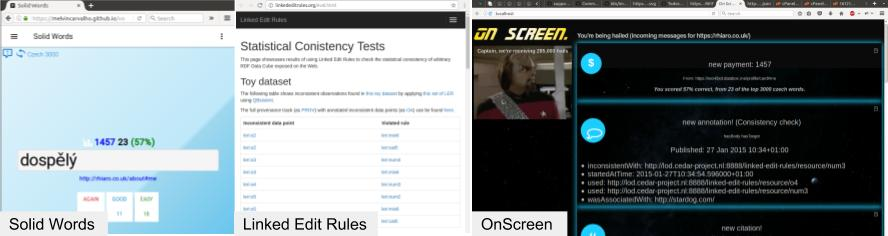
\includegraphics{media/images/screenshot-ldn-sloph-dokieli.jpg}

A \emph{Like} notification created by sloph, displayed by dokieli.

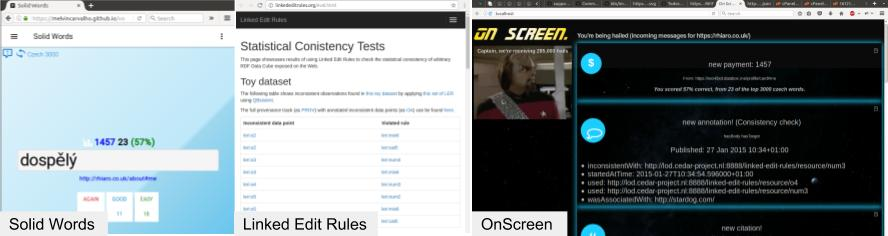
\includegraphics{media/images/screenshot-ldn-senders.jpg}

A: Solid Words (a sender), B: Linked Edit Rules (a sender), C: OnScreen
(a consumer) displaying notifications sent by A and B.

\hypertarget{analysis-and-evaluation}{}
\hypertarget{analysis-and-evaluation}{\subsection{Analysis and
Evaluation}\label{analysis-and-evaluation}}

The LDN protocol describes the discovery of a resource's Inbox whence
notifications are sent or consumed, and the sending and exposure of
those notifications. Here we analyse how well features of LDN achieve
the
\protect\hyperlink{requirements-and-design-considerations}{requirements}
identified previously, and compare this to related work.

We have already examined
\protect\hyperlink{implementations}{implementations} of the
specification and described how they interoperate with each other; this
can be further tested by running the
\href{https://linkedresearch.org/ldn/tests/}{test suite}:
https://linkedresearch.org/ldn/tests/. We can use this towards an
evaluation of its feasibility and effectiveness at interoperability.
Given the relatively early stage in the standardisation process (LDN
entered Candidate Recommendation in 2016-11), the fast adoption of the
LDN specification, quantity of the implementations, and their diversity
is promising and further shows LDN's feasibility. Furthermore, during
the development of the specification issues have been raised or
discussed by 28 different people (excluding the authors; 21 outside of
the Social Web Working Group, 7 within) and the specification has
undergone formal review by internationalisation, accessibility, and
security specialists. We also discuss in more depth particular
challenges that were raised and resolved as part of this process.

\hypertarget{comparison-summary}{}
\subsubsection{Comparison summary}\label{comparison-summary}

Here we compare existing notification mechanisms from related work. The
criteria includes our
\protect\hyperlink{requirements-and-design-considerations}{requirements
and design considerations} (\emph{Rx}) along with additional technical
information which helps to capture some design differences (\emph{Tx}).

Comparison of notification mechanisms

Mechanism

T1

T2

T3

R1

R2

R3

R4-A

R4-B

R4-C\textsuperscript{p}

R4-C\textsuperscript{v}

R4-C\textsuperscript{o}

R5

\begin{description}
\tightlist
\item[T1]
Notification type
\item[T2]
Delivery method
\item[T3]
Dependencies
\item[R1]
Modularity (application classes: S Sender, R Receiver, C Consumer, U
Subscriber/User)
\item[R2]
Reusability
\item[R3]
Persistence - required? how?
\item[R4-A]
Target representation
\item[R4-B]
Notification body
\item[R4-C\textsuperscript{p}]
Payload processing required?
\item[R4-C\textsuperscript{v}]
Verification - required? how?
\item[R4-C\textsuperscript{o}]
Requirements for referenced resources?
\item[R5]
Subscription
\end{description}

\begin{center}\rule{0.5\linewidth}{\linethickness}\end{center}

\begin{description}
\tightlist
\item[--]
not applicable, out of scope
\item[/]
not specified, in scope
\item[X]
explicitly disallowed
\item[app]
application specific decision
\item[!]
required (\emph{MUST})
\item[+]
recommended (\emph{SHOULD})
\item[O]
optional (\emph{MAY})
\item[PuSH]
PubSubHubbub
\end{description}

\begin{center}\rule{0.5\linewidth}{\linethickness}\end{center}

\begin{description}
\tightlist
\item[\textsuperscript{h}]
HTML recommended
\item[\textsuperscript{j}]
Alternate RDF formats can be negotiated
\item[\textsuperscript{k}]
\texttt{source} and \texttt{target} key--value pairs is required
\item[\textsuperscript{q}]
Provenance records with \href{http://www.w3.org/TR/prov-o/}{PROV
Ontology}
\item[\textsuperscript{r}]
RDF representation recommended
\item[\textsuperscript{ra}]
SPARQL results transformed to RSS/Atom
\item[\textsuperscript{s}]
\href{https://www.sitemaps.org/protocol.html}{Sitemaps}
\item[\textsuperscript{t}]
Described in an RDF store or dataset
\end{description}

Semantic Pingback

Linkback

POST

RDF

S R

/

/

Any\textsuperscript{r}

form urlencoded\textsuperscript{k}

!

! parse source

Any\textsuperscript{r}

X

Webmention

Linkback

POST

HTML

S R

--

--

Any\textsuperscript{h}

form urlencoded\textsuperscript{k}

!

! parse source

Any\textsuperscript{h}

X

Provenance Pingback

Linkback

POST

RDF

S R

/

/

/

URI list

/

/

RDF\textsuperscript{q}

X

DSNotify

Fat ping

POST, PUT

XML, PuSH

S U

/

--

--

XML

/

--

RDF\textsuperscript{t}

!

sparqlPuSH

Fat ping

POST

XML, SPARQL, PuSH

S U

--

--

--

XML\textsuperscript{ra}

/

--

RDF\textsuperscript{t}

!

ResourceSync

Fat ping

POST

XML, PuSH

S U

/

--

--

XML\textsuperscript{s}

/

--

?

!

Linked Data Notifications

Fat ping

POST

JSON-LD

S R C

!

! URI

Any

JSON-LD\textsuperscript{j}

+ app

+ app

--

O app

Given that each application requires to follow the steps listed in
``\protect\hyperlink{sender-to-receiver}{Sender to receiver
interaction}'' and ``\protect\hyperlink{consumer-to-receiver}{Consumer
to receiver interactions}'' the metrics are dependent on the performance
of client and server to do HTTP requests and responses, and their
respective payloads.

\hypertarget{compatibility-with-existing-systems}{}
\subsubsection{Compatibility with existing
systems}\label{compatibility-with-existing-systems}

Per \protect\hyperlink{modularity}{R1} and
\protect\hyperlink{adaptability}{R4} we have tried to optimise LDN for
use as a module of a larger system. The success of this is demonstrated
by implementations which use LDN alongside existing protocols according
to their specific needs.

The Solid suite of tools, Virtuoso+ODS-Briefcase, and dokieli use
\href{https://www.w3.org/wiki/WebAccessControl}{Web Access Control}
along with an authentication mechanism to apply fine grained access
controls to restrict who can send notifications, or who can retrieve
notifications from the Inbox. sloph demonstrates an Inbox as a
\href{http://www.webhooks.org/}{Webhooks} callback URL, for requesting
notifications from APIs which post JSON-based payloads.
\href{https://www.w3.org/TR/activitypub/}{ActivityPub} is a W3C CR for
decentralised social media {[}\protect\hyperlink{ref-19}{19}{]}. It uses
LDN for delivery of notifications with the
\href{https://www.w3.org/ns/activitystreams-vocabulary}{ActivityStreams
2.0} (AS2) vocabulary, and specifies additional specialised receiver
behaviour; also used by sloph. dokieli uses the
\href{https://www.w3.org/TR/annotation-protocol/}{Web Annotation
Protocol}, an LDP-based mechanism for creating new content, which acts
as a trigger for notifications to be sent to the Inbox of the annotation
target. The \href{http://fcrepo.github.io/fcrepo-specification/}{Fedora
API Specification} is in the process of being formalised (as an
extension of LDP) by the Fedora community. The repository event stream
draws upon the LDN specification, allowing LDN consumers and senders to
react asynchronously to repository events.

Any existing LDP implementation can serve as an LDN receiver. Simply
advertising any \texttt{ldp:Container} as the Inbox for a resource is
sufficient. We confirmed this with four LDP servers which were developed
independently with different code bases, prior to the LDN specification
(CarbonLDP, Fedora Commons, Solid Server, Virtuoso).

LDN has been integrated into existing domain specific systems: dokieli,
Fedora Commons, IndieAnndroid, Linked Edit Rules, sloph, solid-client,
Solid Words. Standalone implementations of LDN are also straightforward
as a result of this modularity, ie: errol, mayktso, onscreen, pyLDN,
RDF-LinkedData-Notifications, solid-inbox, solid-notifications.

\hypertarget{optimising-implementation}{}
\subsubsection{Optimising
implementation}\label{optimising-implementation}

{We have considered tradeoffs between the HTTP operations receivers and
publishers are \emph{required} to respond to, and ways in which
developers may wish to optimise senders or consumers by reducing
outbound requests.}

{{\texttt{HEAD} requests are low cost, and \texttt{GET} requests may be
high cost if the body of the resource is large.}} {{Given that an Inbox
may be discovered from the HTTP headers of a resource, senders and
consumers can optimise by attempting a \texttt{HEAD} request for
discovery, and only continuing with a \texttt{GET} request if the
\texttt{HEAD} is not successful. On the other hand, senders and
consumers may be attempting discovery upon RDF resources which they
already intend to parse into their own storage. In this case, there is
no need for a \texttt{HEAD} request, as a \texttt{GET} will yield both
HTTP \texttt{Link} headers and an RDF body, either of which could
include the Inbox triple. This means that resources advertising an Inbox
must respond to \texttt{GET} requests (even if only with HTTP headers)
and may respond to \texttt{HEAD} requests.}}

\hypertarget{data-formats}{}
\subsubsection{Data Formats and Content
Negotiation}\label{data-formats-and-content-negotiation}

{Handling data irrespective of the particular RDF serialisation permits
some flexibility, but can be costly to support. We take into account:
(a) application interoperability, (b) maintenance of RDF parsers and
serialisation libraries, (c) complexity of their inclusion in
applications, (d) run-time efficiency.}

{{To address these issues, LDN requires all applications to create and
understand the JSON-LD syntax, both for the contents of Inbox as well as
for individual notifications. Choosing a single serialisation to
\emph{require} is necessary for consistent interoperability, as well as
keeping processing requirements or external code dependencies minimal.}}
{{JSON-LD is advantageous in being familiar for developers who are
\href{http://manu.sporny.org/2014/json-ld-origins-2/}{used to JSON-based
APIs but not RDF} {[}\protect\hyperlink{ref-20}{20}{]}, and it is
compatible with existing JSON libraries or in some cases native
programming language data structures.}}

Optionally, {{applications may attempt to exchange different RDF
serialisations by performing content negotiation}} ({{receivers can
expose \texttt{Accept-Post} headers for senders, and consumers can send
\texttt{Accept} headers to receivers}}).

\hypertarget{precision}{}
\subsubsection{Precision}\label{precision}

In placing no constraints on the contained information, LDN enables a
sender to be precise and lossless with the data it is transmitting.
Approaches which send only URLs rely on the receiver interpreting a
third-party resource, which may or may not contain structured markup or
be under the control of the sender. Approaches which offer additional
guidance to aid the receiver in interpreting the source document(s)
nonetheless still restricts the sender. LDN therefore offers flexibility
to senders, increasing the potential uses for the notification
mechanism. LDN compensates for increased complexity on the receiver's
end by recommending filtering mechanisms, and moving some of the burden
of understanding notifications to the consumer role. As such LDN can
cover a broader variety of use cases.

\hypertarget{accommodating-different-targets}{}
\subsubsection{Accommodating different
targets}\label{accommodating-different-targets}

Per \emph{R4 Adaptability}, we want LDN to be available for all
resources in any publishing context. We consider lowering the bar for
publishers of target resources to be a worthwhile trade-off against
slightly increased complexity for senders and consumers. This is why we
require that senders and consumers must be equipped to discover Inboxes
through both HTTP headers and RDF content.

Since binary formats such as images and video cannot contain an RDF
relation, the HTTP header is essential for including them. It also
allows the inclusion of resources for which it is undesirable or
impractical to add individual Inbox relations, such as to elements in a
dataset; or circumstances where the developer responsible for the Inbox
relation is unable to modify the content. Conversely, non-informational
resources (represented with fragment URIs or 303 redirects) are unable
to express HTTP headers. Their relation to an Inbox must be expressed in
an RDF source. However, if a sender or consumer has a domain-specific
requirement to \emph{only} ever target non-informational resources, they
are exempt from the requirement of discovery via HTTP headers.

\hypertarget{conclusions}{}
\subsection{Conclusions}\label{conclusions}

In this article we describe LDN, a protocol for decentralised semantic
notifications, currently undergoing standardisation at the W3C. Key
elements are:

\begin{itemize}
\tightlist
\item
  Notifications as retrievable, reusable entities with their own URIs.
\item
  Distinct conformance classes for senders, receivers, and consumers.
\item
  Deliberately not defining the vocabulary of notification contents to
  allow for use in a range of different application domains.
\item
  Flexibility of authentication and verification, for the same reason.
\end{itemize}

We outlined design requirements, describe how LDN meets these, and
compare this with related work. We consider LDN to have greater
modularity and adaptability to different scenarios, as well as good
conformance with Linked Data principles. This specification has
potential to have high impact in increasing interoperability between
decentralised Linked Data applications in related domains, as well as
generating new discoverable content for the LOD Cloud. This is evidenced
by 17 diverse implementations which can be shown to interoperate with
each other, including generic libraries and datastores, and
domain-specific applications. Being on the W3C standards track increases
the likelihood of further adoption.

\hypertarget{references}{}
\subsection{References}\label{references}

\begin{enumerate}
\item
  \hypertarget{ref-1}{}

  Mansour, E., Sambra, A., Hawke, S., Zereba, M., Capadisli, S., Ghanem,
  A., Aboulnaga, A., Berners-Lee, T.: A Demonstration of the Solid
  Platform for Social Web Applications, WWW, Demo, 2016,
  \url{http://www2016.net/proceedings/companion/p223.pdf}
\item
  \hypertarget{ref-2}{}

  Tramp, S., Frischmuth, P., Ermilov, T., Shekarpour, S., Auer, S.: An
  Architecture of a Distributed Semantic Social Network, Semantic Web
  Journal, 2012,
  \href{http://www.semantic-web-journal.net/sites/default/files/swj201_4.pdf}{}
\item
  \hypertarget{ref-3}{}

  Arndt, N., Junghanns, K., Meissner, R., Frischmuth, F., Radtke, N.,
  Frommhold, M., Martin, M.: Structured Feedback, WWW, LDOW, 2016,
  \url{http://events.linkeddata.org/ldow2016/papers/LDOW2016_paper_02.pdf}
\item
  \hypertarget{ref-4}{}

  Capadisli, S., Guy, A.: Linked Data Notifications, W3C Candidate
  Recommendation, 2016, \url{https://www.w3.org/TR/ldn/}
\item
  \hypertarget{ref-5}{}

  Parecki, A.: Webmention, W3C Proposed Recommendation, 2016,
  \url{https://www.w3.org/TR/webmention/}
\item
  \hypertarget{ref-6}{}

  Langridge, S., Hickson, I.: Pingback 1.0, 2002,
  \url{http://www.hixie.ch/specs/pingback/pingback}
\item
  \hypertarget{ref-7}{}

  Klyne, G., Groth, P.: PROV-AQ: Provenance Access and Query, W3C Note,
  2013, \url{http://www.w3.org/TR/prov-aq/}
\item
  \hypertarget{ref-8}{}

  Haslhofer, B., Popitsch, N.: DSNotify -- Detecting and Fixing Broken
  Links in Linked Data Sets, WWW, 2010,
  \url{http://eprints.cs.univie.ac.at/81/1/2010_WWW_DSNotify.pdf}
\item
  \hypertarget{ref-9}{}

  Passant, A., Mendes, P.N.: sparqlPuSH: Proactive notification of data
  updates in RDF stores using PubSubHubbub, SFSW, CEUR Workshop
  Proceedings, Vol. 699, 2010,
  \url{http://ceur-ws.org/Vol-699/Paper6.pdf}
\item
  \hypertarget{ref-10}{}

  Klein, M., Van de Sompel, H., Warner, S., Klyne, G., Haslhofer, B.,
  Nelson, M., Lagoze, C., Sanderson, R.: ResourceSync Framework
  Specification -- Change Notification, 2016,
  \url{http://www.openarchives.org/rs/notification/1.0/notification}
\item
  \hypertarget{ref-11}{}

  Berners-Lee, T.: Cool URIs don't change, W3C, 1998,
  \url{https://www.w3.org/Provider/Style/URI.html}
\item
  \hypertarget{ref-12}{}

  Archer, P., Loutas, N., Goedertier S., Kourtidis, S.: Study On
  Persistent URIs, 2012,
  \url{http://philarcher.org/diary/2013/uripersistence/}
\item
  \hypertarget{ref-13}{}

  Fielding, R. T.: Architectural Styles and the Design of Network-based
  Software Architectures. Doctoral dissertation, University of
  California, Irvine, 2000,
  \url{http://www.ics.uci.edu/~fielding/pubs/dissertation/rest_arch_style.htm}
\item
  \hypertarget{ref-14}{}

  Page, K.R., De Roure, D.C., Martinez, K.: REST and Linked Data: a
  match made for domain driven development?, WWW, WS-REST, 2011,
  \url{http://ws-rest.org/2011/proc/a5-page.pdf}
\item
  \hypertarget{ref-15}{}

  Knublauch, H., Kontokostas, D.: Shapes Constraint Language, W3C
  Working Draft, 2016, \href{https://www.w3.org/TR/shacl/}{}
\item
  \hypertarget{ref-16}{}

  Speicher, S., Arwe, J., Malhotra, A.: Linked Data Platform, W3C
  Recommendation, 2015, \url{https://www.w3.org/TR/ldp/}
\item
  \hypertarget{ref-17}{}

  Capadisli, S., Guy, A., Auer S., Berners-Lee, T.: dokieli, 2016,
  \url{http://csarven.ca/dokieli}
\item
  \hypertarget{ref-18}{}

  Snell, J., Prodromou, E.: Activity Streams 2.0, W3C Candidate
  Recommendation, 2016,
  \url{https://www.w3.org/TR/activitystreams-core/}
\item
  \hypertarget{ref-19}{}

  Webber, C., Tallon, J.: ActivityPub, W3C Candidate Recommendation,
  2016, \url{https://www.w3.org/TR/activitypub/}
\item
  \hypertarget{ref-20}{}

  Sporny, M.: JSON-LD and Why I Hate the Semantic Web, 2014,
  \url{http://manu.sporny.org/2014/json-ld-origins-2/}
\end{enumerate}

\end{document}
